\documentclass[12pt]{article}
\usepackage{url}
\usepackage{amsmath}
\usepackage{amsfonts}
\usepackage{graphicx}
\usepackage{listings}
\graphicspath{ {./img/} }

\setlength\parindent{0pt}

\begin{document}

\title{Notes on Groth16}

\section*{Overview}

These notes briefly describe a zk-SNARK construction, and its
use of elliptic curve pairings and a common reference string for
non-interactivity. This is largely based off of 
\url{https://electriccoin.co/blog/snark-explain/}. Relevant papers:
\url{https://eprint.iacr.org/2016/260.pdf}(Groth16) and
\url{https://eprint.iacr.org/2013/279.pdf}(Pinocchio).\\

This schematic shows how we transform the computation.\\ 


\begin{tabular}{ l }
  Computation \\
  Arithmetic Circuit \\
  Rank 1 Constraint System \\
  Quadratic Arithmetic Program \\
  Non-interactive Linear Proof \\
  Non-interactive Zero Knowledge Argument
\end{tabular}



\section*{Arithmetic Circuit}


\begin{figure}[h]
  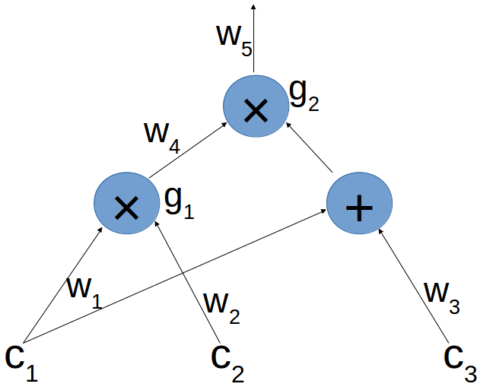
\includegraphics[width=0.5\textwidth]{circuit}  
  \caption[Circuit]{Image from https://electriccoin.co/blog/snark-explain5/}
  \label{fig:circuit}
\end{figure}

The first step is to convert whatever problem on hand into 
a form that can be checked by an arithmetic circuit 
(something with inputs to addition and multiplication gates only).
The circuit in the above diagram allows Alice to prove to 
Bob that she knows some $a_1, a_2$ and $a_3$ such that
$(a_1\cdot a_2)\cdot(a_1+a_3) = 7$

N.B. NP-complete problems are the ``hardest'' problems in NP and we can
convert a problem in NP to one in NP-complete (i.e. transform a problem 
into an arithmetic circuit)


\section*{Rank 1 Constraint System}

The next step is to convert each gate to a constraint

The variables are as follows:
\begin{itemize}
\item $n$: number of multiplication gates (constraints)
\item $m$: number of circuit inputs (size of witness)
\item $u$: left input, $v$: right input, $w$: output 
\end{itemize}

For example: variable mapping is $(1, a_1, a_2, a_3, a_1.a_2, a_1+a_3)$,
at the first gate, we have:
\begin{align*}
u_1 = (0, 1, 0, 0, 0, 0)\\
v_1 = (0, 0, 1, 0, 0, 0)\\
w_1 = (0, 0, 0, 0, 1, 0)
\end{align*}

(note that the first variable is always set to 
1 to allow us to handle constants (affine transformations))

\begin{align*}
\left(\sum_{i=0}^m a_i u_{i,q}\right)
\left(\sum_{i=0}^m a_i v_{i,q}\right)
=
\left(\sum_{i=0}^m a_i w_{i,q}\right)
\end{align*}

$q$ runs over the constraints, so we have $n$ of these equations.


A more sophisticated example is from the comparator 
example in the directory. We can view the constraints
as follows. Try compiling 

\begin{lstlisting}[language=bash]
  $ cd comparator
  $ cp force_equal_if_enabled.circom circuit.circom 
  $ circom circuit.circom
  $ snarkjs printconstraints
\end{lstlisting}

Can you draw a diagram of the circuit represented by the 
three constraints?

\section*{Quadratic Arithmetic Programs}

\begin{align*}
  u_i(r_q) &= u_{i,q}, \quad\\
  v_i(r_q) &= v_{i,q}, \quad\\
  w_i(r_q) &= w_{i,q}, \quad\\
  \left(\sum_{i=0}^m a_i u_i(X)\right)\left(\sum_{i=0}^m a_i v_i(X)\right)
           &= \left(\sum_{i=0}^m a_i w_i(X)\right) \mod t(X)
\end{align*}

Now use Lagrange interpolation to encapsulate the R1CS information as polynomials:
Note that the polynomial will be evaluated at $n$ points
In words, each of the constraints is now represented by the evaluation of 
this constraint polynomial at a particular point $r_q$. Now the verifier can check by multiplying 
the $(a_0, a_1, ..., a_n)$ vector with the polynomials in one step.\\

N.B. A Lagrange basis polynomial for a particular point $x_i$ is one 
that is chosen to be 1 at that particular point and 0 at all other points.

\section*{Non-interactive linear proof}

Useful fact: Schwarz-Zippel lemma - consider a polynomial in $n$ variables over a field $K$. Pick $n$ random points in $K$ to evaluate this polynomial, probability of this evaluating to zero is at most the degree divided by the cardinality of the field. (proof by induction on $n$)\\

Preliminary sketch of an interactive protocol -
\begin{itemize}
\item Alice wants to prove to Bob that she has a satisfying assignment
  to a polynomial she commits to:
\item 
  Alice chooses polynomials $u, v, w, h$ such that $u\cdot v = w + t\cdot h$, all of
  degree at most $d$
  
\item 
  Bob chooses random $s$ in $\mathbb{F}_p$ and computes $E(t(s))$
\item
  Alice sends the encrypted values $E(u(s)), E(v(s)), E(w(s)), E(h(s))$
  Bob checks that the equation holds at $s$, i.e.
  $E(u(s)\cdot v(s)-w(s)) = E(t(s)\cdot h(s))$

\end{itemize}

The following are some gory details to make sure things are watertight.

\subsection*{Ensure polynomials are chosen according to an assignment}

If we just check 
$u(s)\cdot v(s)-w(s) = t(s)\cdot h(s)$
where $u, v, w, h$ are all of degree at most $d$, we 
don't know that $u, v, w$ were constructed from 
a satisfying assignment $(a_1, \dots, a_n)$.

One idea is to combine the polynomials:

\begin{align*}
f_i = u_i + X^{d+1}.v_i + X^{2(d+1)}.w_i
\end{align*}

So Bob will ask Alice to prove to him that $f$ is a linear combination 
of $f_i$'s. He chooses a random $\beta \in \mathbb{F}p^*$ and sends 
hidings $E(\beta\cdot F_1(s)), \dots, E(\beta\cdot F_m(s))$. 
Alice is to respond with $E(\beta\cdot F(s))$ where 
$
F = \sum_{i=1}^m c_i\cdot F_i
$

\subsection*{Concealing the assignment}

(Add a random multiple of $t(X)$ to each of $u, v, w$ to conceal 
information about the assignment used by Alice)


\subsection*{Pairings on elliptic curves}

Consider computing  $E(h(s)\cdot t(s))$ from $E(h(s)$ and $E(t(s))$.\\

The pairing $e: G_1 \times G_2 \rightarrow G_T$, where
the groups are all of prime order $p$, has the property that
$e(a\cdot g, b\cdot h) = e(g, h)^{ab}$.\\

With $E_1(x) = x\cdot g$,
$E_2(y) = y\cdot h$, $E(xy)$ can be constructed with this pairing.

\subsection*{Using a Common Reference String(CRS) for non-interactivity}

Publish Bob's first message as the CRS, i.e.

\begin{align*}
  (E_1(1), E_1(s), \dots, E_1(s^d), E_2(\alpha), E_2(\alpha s), \dots,
  E_2(\alpha s^d))
\end{align*}


TODO: \\
More notes on where the Pairings come from (algebraic geometry)
Resources on Probabilistically Checkable Proofs



\end{document}
